\documentclass[letterpaper]{article}
\usepackage{multirow,graphicx,geometry,hyperref}
\usepackage[listings]{tcolorbox}
\usepackage[sfdefault]{inter} %% Option 'sfdefault' only if 'inter' is to be
\usepackage[T1]{fontenc}
\tcbuselibrary{breakable}
\lstset{tabsize=1,showstringspaces=false,breaklines=true,
        showstringspaces=false,basicstyle=\footnotesize}
\geometry{letterpaper, left=20mm, right=20mm, top=20mm, bottom=20mm}

\tcbset{
  base/.style={
    arc=0mm,
    bottomtitle=0.5mm,
    boxrule=0mm,
    colbacktitle=black!10!white,
    coltitle=black,
    fonttitle=\bfseries,
    left=4mm,
    leftrule=1mm,
    right=3.5mm,
    title={#1},
    toptitle=0.75mm,
  }
}

\definecolor{brandcolor}{rgb}{0.94, 0.7, 1}

\newtcolorbox{mainbox}[1]{
  colframe=brandcolor,
  breakable,
  base={#1},
}

\newtcolorbox{subbox}[1]{
  colframe=black!30!white,
  breakable,
  base={#1},
}

\newenvironment{answer}
  {\par\smallskip\begingroup\leftskip=1em\noindent\ignorespaces}
  {\par\endgroup}

\begin{document}

\hfill
\begin{tabular}{llr}
	\multirow{5}{6em}{\includegraphics[width=2cm]{../../../../../engineering-logo.png}} & {\bf Course:} 	& ENR 452L			    \\
																		    	        & {\bf Assignment:} & Lab 01			    \\ 
																		    	        & {\bf Name:} 		& Anthony Aglieco 	    \\
																		    	        & {\bf Email:} 		& apaglieco1@umary.edu 	\\
																		    	        & {\bf Date:} 		& \today			    \\
\end{tabular}

\bigskip


\section{Assigned questions}

\begin{enumerate}
    \item \textbf{What value did you assign \texttt{\_estack} in your linker file?}
    
\begin{answer}
    \texttt{\_estack} was set to \texttt{0x24080000} for the M7 and \texttt{0x30020000} for the M4.
\end{answer}
    
    \item \textbf{What value did you assign for the Flash Location and Length in your linker file?}
            
\begin{answer}
    The flash address is \texttt{0x08000000} on the M7 and \texttt{0x08100000} on the M4. Both have a length of 1024~KiB.
\end{answer}
    
    \item \textbf{What value did you assign for the RAM Location and Length in your linker file?}
        
\begin{answer}
    The RAM address is \texttt{0x24000000} on the M7 (with a length of 512~KiB) and \texttt{0x30000000} on the M4 (with a length of 128~KiB).
\end{answer}
    
    \item \textbf{What value did you assign to the \texttt{r7} register in the \texttt{reset\_handler.s} file?}
        
\begin{answer}
    On the M7 core, \texttt{0xC0FFEE}. On the M4, \texttt{0xFACADE}.
\end{answer}
    
    \item \textbf{What assembly instruction did you use for incrementing your counting register?}
    
\begin{answer}
    The ARM thumb spec defines the instruction \texttt{ADDS} to add an immediate value to a register while updating appropriate flags.
\end{answer}
    
    \item \textbf{In which documents did you find this information? page?}
        
\begin{answer}
    ARM publishes a \href{https://support.arm.com/documentation/qrc0006/e/}{"quick reference card"} for their thumb instruction set. The \texttt{ADDS} instruction is located on page 1 of this document.
\end{answer}
    
    \item \textbf{In the linker files, you assign the RAM memory size and location that your program will use. \\
          If you have one program running on the Cortex-M4 MCU and one program running on the \\
          Cortex-M7 MCU, what change would you have to make to the linker files?}
            
\begin{answer}
    The programs would have to use different registers, different areas of flash, and different areas of RAM.
\end{answer}

\end{enumerate}

\section{Running the code}

As shown in Figures~\ref{fig:m7-1} and~\ref{fig:m7-2}, the M7 core was loaded with a copy of the \texttt{reset\_handler.s} script.
This was executed, and stopped when \texttt{r0} was at \texttt{0x252ddbd}, started again, and stopped when \texttt{r0} reached \texttt{0x5cd2e6a}.
A similar process was completed for the M4 core, except using \texttt{r1} to count, and stopping at \texttt{0x252dc3b} and \texttt{0x441cd03}. This is shown in Figures~\ref{fig:m4-1} and~\ref{fig:m4-2}.

\begin{figure}[h!]
\begin{center}
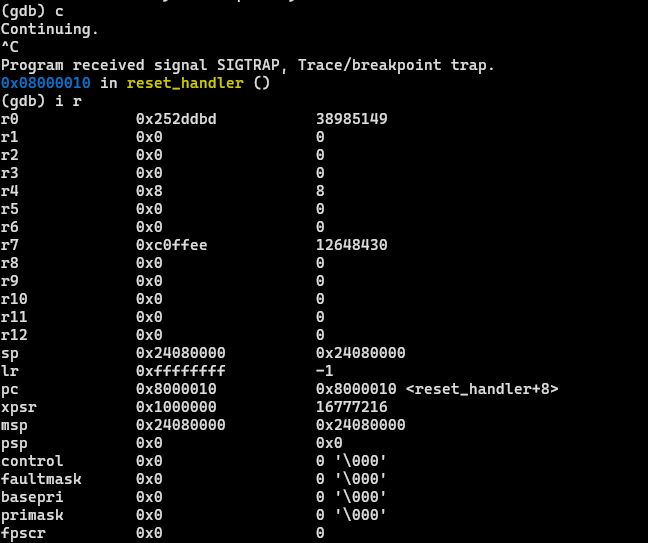
\includegraphics[width=10cm]{./m7-counter-1.png}
\end{center}
\caption{First snapshot of the registers while running a program on the M7 core.}
\label{fig:m7-1}
\end{figure}

\begin{figure}[h!]
\begin{center}
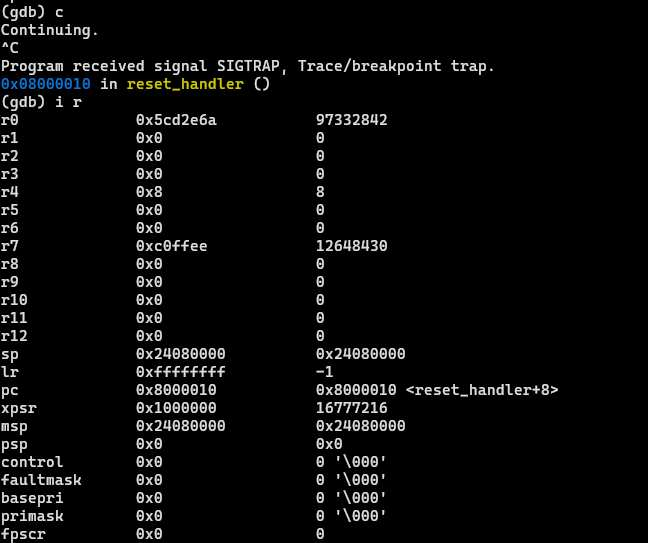
\includegraphics[width=10cm]{./m7-counter-2.png}
\end{center}
\caption{Second snapshot of the registers while running a program on the M7 core.}
\label{fig:m7-2}
\end{figure}


\begin{figure}[h!]
\begin{center}
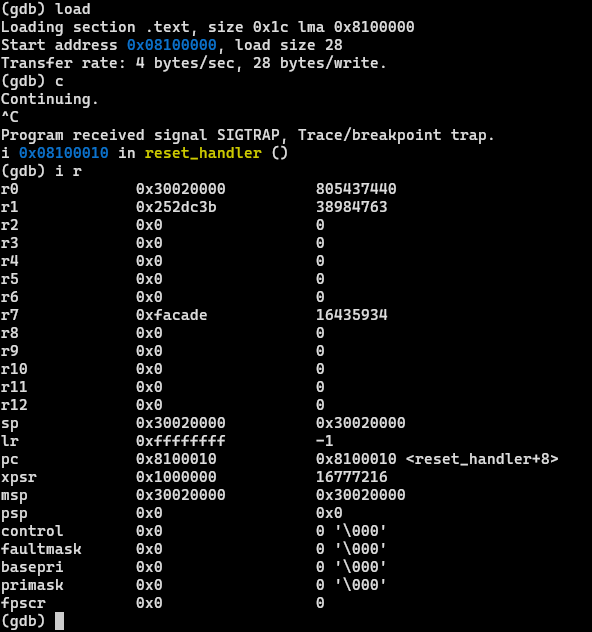
\includegraphics[width=10cm]{./m4-counter-1.png}
\end{center}
\caption{First snapshot of the registers while running a program on the M4 core.}
\label{fig:m4-1}
\end{figure}

\begin{figure}[h!]
\begin{center}
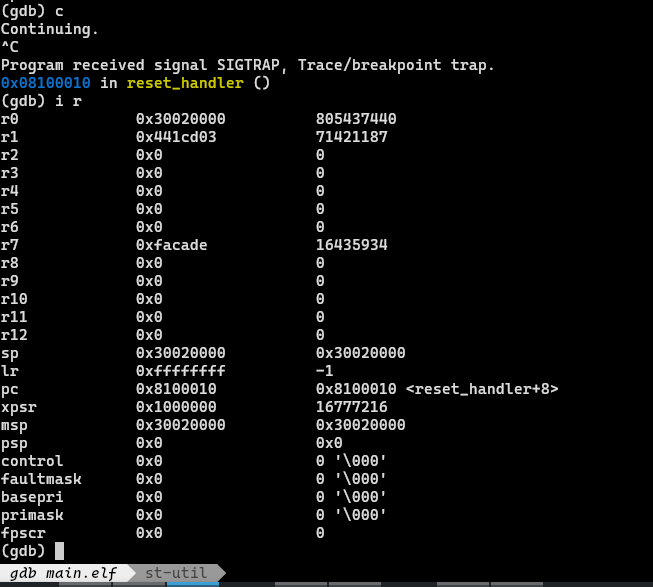
\includegraphics[width=10cm]{./m4-counter-2.png}
\end{center}
\caption{Second snapshot of the registers while running a program on the M4 core.}
\label{fig:m4-2}
\end{figure}

% \section{Exercise 2}
% Furthermore, Exercise 2 was completed using the following steps:


% \subsection{Parts A and B}

% Parts A and B were completed by creating anonymous functions with the appropriate parameters, as seen below.
% \begin{mainbox}{\texttt{ex2.m}}
%     \begin{lstlisting}
% ## part a
% a = @(t) 2.5.*cos(2*pi.*t);
% ## part b
% b = @(t) 2.5.*sin(2*pi.*t);
%     \end{lstlisting}
% \end{mainbox}
% \bigskip\noindent
% For the sake of completeness, the entire script \texttt{ex2.m} is shown below.
% \begin{mainbox}{\texttt{ex2.m}}
%     % \texttt{\lstinputlisting{./ex2.m}}
% \end{mainbox}
\end{document}
